\documentclass[12pt]{article}

\usepackage{setspace}
\usepackage[margin=1in]{geometry}
\usepackage{xeCJK}
\usepackage{fontspec}
\setCJKmainfont[BoldFont={STHeiti}]{FandolSong}
\usepackage{indentfirst}
\usepackage{graphicx}
\usepackage[figurename=图]{caption}

\onehalfspacing
\setlength{\parindent}{24pt}

\newcommand{\enabstractname}{Abstract}
\newcommand{\cnabstractname}{摘要}
\newenvironment{enabstract}{%
  \par
  \mbox{}\hfill{\bfseries \enabstractname}\hfill\mbox{}\par
  \vskip 2.5ex}{\par\vskip 2.5ex}
\newenvironment{cnabstract}{%
  \par
  \mbox{}\hfill{\bfseries \cnabstractname}\hfill\mbox{}\par
  \vskip 2.5ex}{\par\vskip 2.5ex}

\title{\textbf{邓小平“南方谈话”与当下的全面深化改革}}
\author{13\quad 张煜豪\quad 光华管理学院\quad 1900015810\quad email:1900015810@pku.edu.cn}
\date{}

\begin{document}

\maketitle

\begin{cnabstract}
    邓小平同志在1992年的“南方谈话”是极其重要的历史性谈话,它为改革开放的继续开展注入了新的动力和思想指引。在中国特色社会主义新时代,我们依然能,且已经从其中汲取启示,并在实践当中建设中国特色社会主义,不断完善和发展中国特色社会主义理论体系。
\end{cnabstract}

\section{引言}
1992年,邓小平同志在武昌、深圳、珠海、上海等地发表了一系列的谈话,史称“南方谈话”。其时,中国正处在改革的停滞期,1989年以来的政治风波使得经济和政治改革的进程受到了严重的阻碍,经济发展的动力也在逐渐消失。许多人对改革进行下去的信心产生了动摇和怀疑。邓小平同志在南方谈话中,对中国的改革开放进程进行了全面的总结,提出了一系列的改革措施,为中国的改革开放进程注入了新的动力,使得中国的改革开放进程重新回到了正轨上来。本文将对邓小平同志的南方谈话进行全面的解读,分析其与当下全面深化改革的关系与对当今的启示。总的来说,小平同志的讲话启示我们,要敢于改革,破除体制机制和思想上的束缚,解放思想,实事求是,才能取得生产力的大发展,才能全面建成社会主义现代化强国。

\section{历史背景}
1978年的十一届三中全会正式拉开了改革开放的序幕,随之而来的是农村和城市在经济方面的大变化:农村实行了家庭联产承包责任制,大幅提高了农民的生产积极性和生产效率,1978-1984年期间,农业的年增长率一度达到了8.8\%左右,是年经济增长率的3倍。\footnote{勃兰特,罗斯基:《伟大的中国经济转型》,第405页}在政策开放后,乡镇集体企业也成为了经济发展的重要力量。而城市经济在经历一系列针对国有企业的改革后也表现出了活力。但与此同时,价格机制的引入也对人们的生活有所冲击,由于生产能力的缺乏和宏观经济的波动?,物价不可避免地出现上涨的趋势。物价“双轨制”下出现的各种倒卖、腐败现象也引发了社会上的不满。来自西方的各种思潮也影响着人们的价值观和情绪。各种矛盾激化的结果是80年代末的政治风波,它使得改革不得不被搁置以稳定局面,国家一度陷入“改革要不要继续下去”的争论当中。

然而,不继续改革开放,经济将要陷入停滞乃至倒退。在这种情况下,原本已经退出政治舞台的邓小平同志再次站了出来,在武昌、深圳、珠海、上海等改革开放的前沿发表了一系列的谈话,史称“南方谈话”,为中国的改革开放进程注入了新的动力。事实上,在《邓小平文选》(第三卷)的目录中可见,邓小平同志在一九八九年以后的观点发表几乎屈指可数。在《改革开放政策稳定,中国大有希望》\footnote{《邓小平文选》(第三卷)第315页}中,他已经表明,自己从领导岗位上悄悄退下来,是为了中国的长远发展和国际形象,并坚持自己提出的干部年轻化的目标。然而,在1992年他再次选择站出来,用自己的影响力推动中国改革开放的继续进行。这说明当时改革的推进已经困难到了一定的程度,而小平同志的这一系列谈话重新开启了改革开放的快速推进,可见其重要性。

\section{“南方谈话”的主要内容}
邓小平同志在“南方谈话”中讨论了关于中国发展前景的一系列问题,并指出了他对于这些问题的看法和路线指引。下面大致总结一下这些谈话的主要内容:

一、改革开放是经济发展、人民生活富裕幸福的保障,虽然“六四”动摇了部分人改革的决心,但恰是前期的改革开放使得人们对国家有了更多的信心,才能够帮助我们度过这一难关。坚持改革开放,让人民对政府的政策有信心,经济才能真正发展起来。\footnote{《邓小平文选》(第三卷),第370-371页}

二、改革开放就要敢作敢为,不要怕所谓“社会主义”和“资本主义”的争论,计划和市场并不是决定社会制度和意识形态的标准。只要有利于生产力发展,有利于消除贫困、消除两极分化、消灭剥削、共同富裕的,就是社会主义的。不能想着一开始就把所有的事情做对,资本主义使用的工具,在调查研究之后可以大胆去尝试,错了及时纠正即可。“必须大胆吸收和借鉴人类社会创造的一切文明成果,吸收和借鉴当今世界各国包括资本主义发达国家的一切反映现代社会化生产规律的先进经营方式、管理方法。”\footnote{《邓小平文选》(第三卷),第373页}当前(指当时)主要的问题是防止“左”,防止搞过于激进的社会主义,重蹈覆辙。通过先富带动后富,先调动发达地区的积极性,再逐步解决区域发展不均衡的问题。尊重对改革的不同意见,不搞争论,用实践证明一切。\footnote{《邓小平文选》(第三卷),第372-378页}

三、科学技术是第一生产力,要搞好科学和教育,关注科学家。\footnote{《邓小平文选》(第三卷),第378页}

四、坚持“两手抓”。一手抓改革开放,一手要打击各种违法犯罪活动。要做好反腐工作,做好法制建设,并且用法制建设做好廉政建设;坚持人民民主专政,防范资产阶级自由化。总的来说,经济建设和政治治理两方面都要搞好。\footnote{《邓小平文选》(第三卷),第378-380页}

五、在党的工作方面,要做好组织建设,培养“革命化、年轻化、知识化、专业化”的领导班子,健全人才培养机制和老干部的退出机制,防止“老人政治”。警惕形式主义和官僚主义。坚持基本路线,防范资产阶级自由化。只有把共产党内部搞好了,中国才能发展好。\footnote{《邓小平文选》(第三卷),第380-382页}

六、在实践中学习马克思主义,贯彻马克思主义。改革开放靠的不是本本主义,而是靠的在实践中摸索(也即我们常说的“摸着石头过河”)尊重人民群众的实践智慧,效果好的经验可以尝试推广。“马克思主义是很朴实的东西,很朴实的道理。”\footnote{《邓小平文选》(第三卷),第382页}

七、社会主义取代资本主义是历史发展的必然规律,我们要坚定对发展社会主义的信心,将中国发展成社会主义强国(建国一百年成为中等发达国家),成为反对霸权主义、维护世界和平与发展的重要力量。\footnote{《邓小平文选》(第三卷),第382-383页}

\section{新时代的全面深化改革与三十年前的“南方谈话”}
回顾邓小平同志三十年前的讲话,依然感觉振聋发聩。这些讲话几乎全面地概括总结了我国在改革开放中遇到的问题和未来依然会遇到的问题,并提出了基本的路线和方法指引。下面将细致论述这些观点和当下全面深化改革开放在多个方面上的关系。

\subsection{解放和发展生产力}
进入新时代后,我国社会的主要矛盾转变为人民群众日益增长的对美好生活的需要和不平衡不充分的发展之间的矛盾。然而,这一转变并不妨碍小平同志的观点对当下发展的指导作用。在社会主义初级阶段,我们依然面临着相似的矛盾、相似的问题。

首先,要解决不平衡不充分发展的问题,依然要靠不断解放和发展生产力。生产力发展不单单是数量上的增加,更是质量上的提升,而质量上的提升正是解决不平衡与不充分所需要的。过去十年,我国深入进行“供给侧结构性改革”,进行产业转型和升级,大力发展服务业,优化产业结构,大力促进了生产力的质量提升。

他进一步提出,科学技术是第一生产力,要发挥科学家的作用。江泽民同志提出“科教兴国”,习近平总书记提出“创新驱动发展战略”,将创新摆在所有工作的核心位置,无疑都是对这一论断的继承和发展。

1978-2007年间,全要素生产率的增长(可视为制度转型和一系列技术发展的总和)是我国实现相对于他国高速经济增长的关键所在,见图1,中国与美国在劳动参与率、资本占产出比值、人力资本水平等方面的比值差异在这三十年间并没有显著的变化,但全要素生产率(TFP)的提高。\footnote{Xiaodong Zhu: Understanding China's Growth: Past, Present, and Future. \textit{Journal of Economic Perspectives}, 31(1): 107-130, 2017.}从经济学实证科学的角度,邓小平同志的理论也进一步得到了验证。而中国经济想要继续保持增长,就要不断地解放和发展生产力,发展科学技术,并改善发展的制度环境,从而提高全要素生产率。

\begin{figure}[h]
\centering
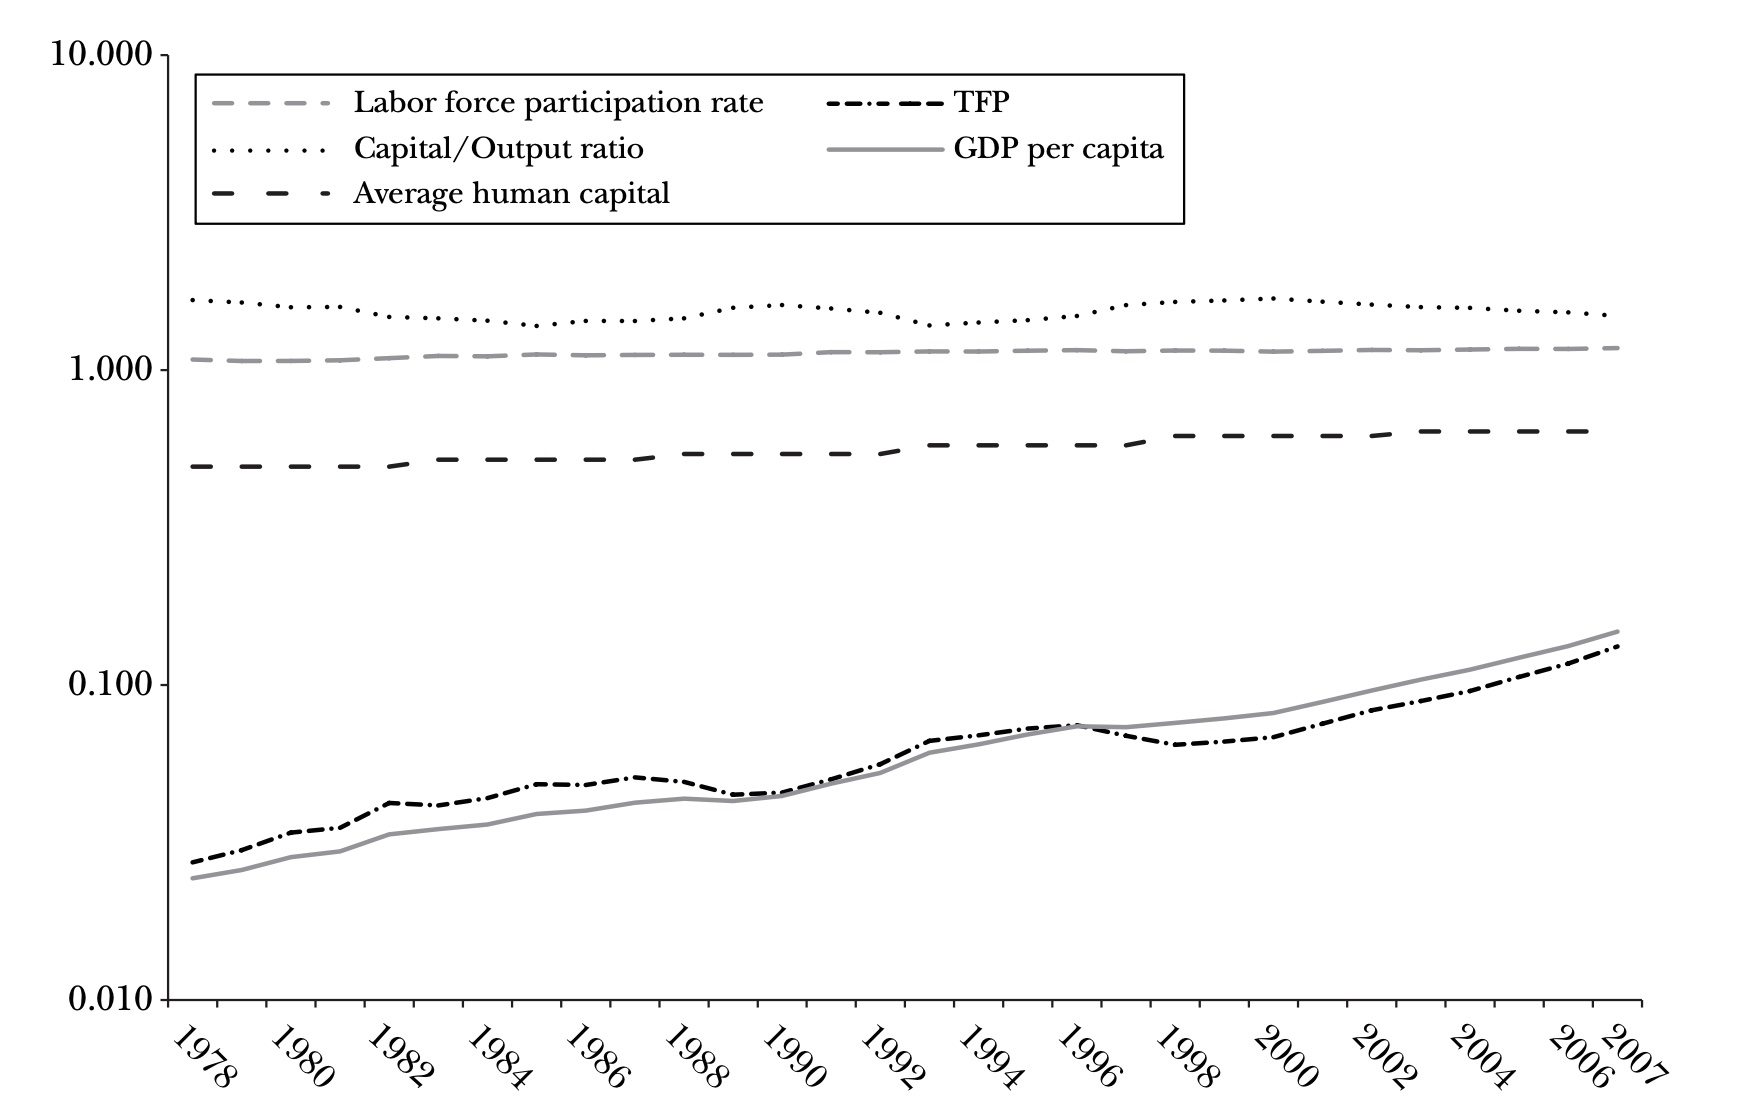
\includegraphics[width=\textwidth]{f1.jpg}
\caption{中国与美国在经济增长方面各项指标的比值}
\begin{flushleft}
  \textit{来源:Xiaodong Zhu (2017)}
\end{flushleft}
\end{figure}

科学技术是第一生产力,不仅意味着要通过不断提升科学技术水平来提升生产力水平,还意味着要努力掌握先进核心技术,不被“卡脖子”,更大程度上实现自给自足。习近平总书记提出加快形成“以国内大循环为主体、国内国际双循环相互促进的新发展格局”,也不断在提升自主性方面作出努力。\footnote{国家发展改革委员会规划司:《推动形成以国内大循环为主体、国内国际双循环相互促进的新发展格局》,2021}

\subsection{法治建设与廉政建设}
在经济发展的过程中,随着逐利机会的涌现,不免会出现许多游走在法律规范边缘乃至违反法律的行为,这种现象发生在中国共产党的干部和政府官员身上,危害尤其严重,是对人民群众利益的损害、对公平法治的无视、对社会秩序的挑衅、对人民政权的合法性的伤害。因此,小平同志在经历了“六四”的风波过后,敏锐地指出了这一点,提出了“两手抓”,不仅要抓普通的违法犯罪,更要抓内部的腐败,做好法制建设。

十八大以来,党中央开展了一系列反腐行动,进行党风廉政建设。据统计,截至2022年4月,全国纪检监察机关共立案审查调查438.8万件、470.9万人\footnote{2022年6月30日中共中央宣传部坚持党的全面领导和全面从严治党新闻发布会},反腐力度空前。2018年,国家监察委员会成立,意味着中国共产党的廉政建设法制化程度迈上了新台阶。坚决的反腐行动能够防止政府成为“掠夺之手”,保障市场秩序的稳定、人民群众的合法权益,并防止社会陷入寻租腐败的氛围和人心的扭曲。小平同志对我国政治治理改革的期望,终于在二十多年后得到更加充分的实现。

十八大以来,我国也不断坚持中国特色社会主义法治体系建设,如2020年5月颁布的《民法典》,终于填补了我国没有民法典的空白,从此人民群众维护自身权益更加有法可依,国家的治理体系与治理能力得以更加现代化。

\subsection{马克思主义的中国化}
除了以上具体的发展路线,邓小平也对马克思主义普遍性原理的中国化提出了自己的见解和创新。马克思主义是活的东西,而不是一成不变的教条。而马克思主义最基本的一则原理,就是真理只有在实践当中才能得到检验。早在十一届三中全会,邓小平同志就提出“解放思想,实事求是”的口号,这是对马克思主义,对毛泽东思想的忠实继承。

我国在改革开放当中形成了一套有中国特色的政策试点推广体系。例如“营改增”的重大改革、司法财政的独立性改革,都是在各个地方先行先试,然后再逐步推广到全国。这种做法,就是在实践当中不断地检验制度设计的正确性,从而形成一套适合中国国情的理论和知识体系。研究表明,改革开放40年来,我国政府进行了至少652项政策试点和推广,其中42\%的政策最终得到了全国性推广。\footnote{Shaoda Wang, David Y. Yang: Policy Experimentation in China: The Political Economy of Policy Learning. \textit{Working Paper}, 2023.}这就是马克思主义科学认识论和实践论的生动体现。邓公说“马克思主义是很朴实的道理”,诚哉斯言。

马克思主义的中国化,就是要把马克思主义的普遍原理同中国革命和建设的具体实际、历史和实践相结合,从而形成一套适合中国国情的理论体系。而邓小平同志一系列看似朴实实则智慧的理论观点,正是马克思主义在中国改革开放初期背景下对发展道路探索的理论升华和指引。

\subsection{什么是社会主义}
从“文化大革命”中走出来的邓小平,深切体会到意识形态争论和过于谨慎敏感的政治态度对于经济发展的阻碍和危害。“六四”过后,这种态度又一次显露出来,对于资产阶级自由化的提防导致束手束脚。因此,他在“南方谈话”中特意指明了“什么是社会主义”的问题:他说,社会主义的本质就是解放和发展生产力,消灭剥削,消除两极分化,实现共同富裕。计划和市场都只是经济手段。这一看似简单的论断搁置了各种各样的争论,为改革开放的顺利开展铺开了道路。

在四十年后的今天,我们依然能从这句话中学到许多。在社会不平等日益扩大和互联网日益发达的今天,我们能看到越来越多不满的声音,有一种“左”的思潮正在日益流行。许多人认为,我国的经济应当更加“社会主义”,适当回归计划经济时代的模式,才能促进公平。然而,小平同志的话告诉我们,所谓社会主义并无成文的发展模式,也未必只有计划经济才能实现消除两极分化的目标。但我们应当反思在消除两极分化方面做的不足的地方:人民群众的公共服务是否实现了均等化?水平是否足够?人民群众是否享有平等和充分的权利?如何解决房价高企的问题?地方政府是否应该摆脱通过高价出售商品房土地解决财政问题的发展模式?无论是怎样的发展手段和模式,我们都应当把社会主义的这几个本质特征牢记在心。

\subsection{国际关系}
最后,邓小平同志也提及了中国改革开放与国际社会之间的关系。他坚持了自己“和平与发展是当今世界的两大问题”的论断,并强调中国的强大要有利于世界的和平与发展,中国要成为与霸权主义对抗的重要力量。

21世纪的中国越来越成为维护世界和平与发展的中坚力量。习近平总书记提出构建人类命运共同体,并通过“一带一路”建设、积极参与解决国际问题等行动实践这一理念。并且,在逆全球化甚嚣尘上,世界矛盾复杂多变的今天,中国更要发挥自己的大国影响力,积极解决世界和平与发展的问题。

\section{反思与补充}
马克思主义中国化是一个不断自我完善、自我扬弃的过程。站在新时代的角度上,我们会发现邓小平同志在谈话中对一些当今突出的问题缺乏讨论。我们应当对邓小平同志的谈话有更新的认识,并基于邓小平理论形成更完善的一套关于社会主义现代化的理论认知,这也正是中国特色社会主义理论体系不断更新完善的过程。

首先,他对于市场体制的改革并没有指出更加明确的方向。当时改革还没有进入深水区,经济增长依然能够通过对价格机制的放开、对国有企业的放活、大力进行投资建设来实现,换句话说,计划经济时期(特别是后期)的经济秩序混乱和低效严重压抑了中国经济增长潜力的实现,改革开放所做的事情很大程度上是帮助这种潜力实现。而在社会主义市场经济体系已经基本建成的今天,我们更加迫切地需要市场和政治制度的完善来保障市场在资源配置中起决定性作用,实现高质量发展和持续的经济增长。过去能够实现的经济增长,而今需要以更加艰难而更加系统性的方式来实现。

社会主义市场经济的建设不只是经济的发展,还是制度的建设,而政府在制度建设和维护当中又起着关键的作用。政府需要保护个人和企业的合法产权,才能充分激发经济主体的活力,从而不断促进创新、促进经济增长。政府需要不断完善产品和要素价格市场化机制,才能更大程度上发挥市场在资源配置中的决定性作用。要打造亲清型政商关系,打造服务型政府,维护市场的公平竞争准入,更好地处理政府与市场之间的关系。

\section{总结}
邓小平理论是马克思主义中国化的重要成果,是指引中国深化改革开放的重要精神财富。而“南方谈话”是邓小平同志留下的最后成果,是他的理论智慧结晶。我们要基于现实不断完善以邓小平理论为代表的中国特色社会主义理论体系,为愈发复杂艰难的改革进程提供思想理论指引。我们要不断坚持中国特色社会主义道路,不断解放和发展生产力,全方位深化改革开放,建设社会主义现代化强国,实现人民富裕、国家富强。

\section*{参考文献}
[1]邓小平. 邓小平文选[M]. 北京:人民出版社,2003.\par
[2]勃兰特,罗斯基,编. 伟大的中国经济转型[M]. 方颖等,译. 上海:格致出版社:上海人民出版社,2009.\par
[3]国务院新闻办公室. 中共中央宣传部举行坚持党的全面领导和全面从严治党新闻发布会图文实录[EB/OL].(2022-06-30)[2023-05-12]. http://www.scio.gov.cn/xwfbh/xwbfbh/w\\qfbh/47673/48442/wz48444/Document/1726239/1726239.htm.\par
[4]国家发展改革委员会规划司. 推动形成以国内大循环为主体、国内国际双循环相互促进的新发展格局[EB/OL].(2021-12-25)[2023-05-12]. https://www.ndrc.gov.cn/fggz/fzzlgh/\\gjfzgh/202112/t20211225\_1309698.html.\par
[5]ZHU Xiaodong. Understanding China's Growth: Past, Present, and Future[J]. {Journal of Economic Perspectives}, 31(1): 107-130, 2017.\par
[6]WANG Shaoda, YANG Y. Policy Experimentation in China: The Political Economy of Policy Learning[R]. Working paper, 2023.



\end{document}